\documentclass[12pt]{article}
\usepackage{amsmath}
\usepackage{amsthm}
\usepackage{amssymb}
\usepackage{euscript}
\usepackage{mathrsfs}
\usepackage{bm}
\usepackage{enumitem}
\usepackage{tikz}
\usepackage{mathtools}
\usepackage{float}
\usepackage{hyperref}
\usepackage{boldline}
\usepackage{indentfirst}
\usepackage{environ}
\usetikzlibrary{positioning}

\hypersetup{
    colorlinks=true,
    linkcolor=[RGB]{0,0,128},
    filecolor=magenta,
    urlcolor=cyan,
    citecolor = [RGB]{128,0,128}
}
\newcommand{\makeBox}[2] {
  \newsavebox{#1}
  \begin{lrbox}{#1}{#2}\end{lrbox}
}

\tikzstyle{tableau} = [y = -1cm, every node/.style={transform shape}]

\definecolor{gridColor}{RGB}{19,83,150}
\tikzstyle{dominoStyle} = [color=black, fill=white, rounded corners = .1cm, thick]
\tikzstyle{gridLine} = [color=gridColor, thick]
\tikzstyle{dominoText} = [font=\Large, midway]
\tikzstyle{cycleLine} = [color=green, thick, >->]
\tikzstyle{closedCycleLine} = [color=green, thick]
% \tikzstyle{fixedSquareStyle} = [pattern = crosshatch doats, pattern color=gridColor,  opacity=0.2]
\tikzstyle{fixedSquareStyle} = [color=gridColor,  opacity=0.07]
\tikzstyle{tileText} = [font=\large, midway]

\newcommand{\eps}{.06}
\newcommand{\teps}{\eps * 2}

% first entry is row, starting with 1, second entry is column, third is content
\newcommand{\filledSquare}[3]{\filldraw [dominoStyle] (#2 - 1 + \eps, #1 - 1 + \eps) rectangle + (1 - \teps, 1 -\teps) node [tileText] {$#3$};}
% The fourth entry shifts vertically
\newcommand{\filledSquareShift}[4]{\filldraw [dominoStyle] (#2 - 1 + #4 + \eps, #1 - 1 + \eps) rectangle + (1 - \teps, 1 -\teps) node [tileText] {$#3$};}

\newcommand{\horizontalDomino}[3]{\filldraw [dominoStyle] (#2 - 1 + \eps, #1 - 1 + \eps) rectangle + (2 - \teps, 1 -\teps) node [dominoText] {$#3$};}
\newcommand{\verticalDomino}[3]{\filldraw [dominoStyle] (#2 - 1 + \eps,  #1 - 1 + \eps) rectangle + (1 - \teps,2 -\teps) node [dominoText] {$#3$};}

\newcommand{\horizontalDominoShift}[4]{\filldraw [dominoStyle] (#2 - 1 + #4 + \eps, #1 - 1 + \eps) rectangle + (2 - \teps, 1 -\teps) node [dominoText] {$#3$};}
\newcommand{\verticalDominoShift}[4]{\filldraw [dominoStyle] (#2 - 1 + #4 + \eps,  #1 - 1 + \eps) rectangle + (1 - \teps,2 -\teps) node [dominoText] {$#3$};}

\newcommand{\zeroSquare}[2]{\filldraw [dominoStyle] (#2 - 1 + \eps, #1 - 1 + \eps) rectangle + (1 - \teps, 1 -\teps) node [dominoText] {$0$};}
\newcommand{\zeroSquareShift}[3]{\filldraw [dominoStyle] (#2 - 1 + #3 + \eps, #1 - 1 + \eps) rectangle + (1 - \teps, 1 -\teps) node [dominoText] {$0$};}


\newcommand{\emptyBox}[2]{\filldraw [dominoStyle] (#2 - 1 + \eps, #1 - 1 + \eps) rectangle + (2 - \teps, 2 -\teps);}
\newcommand{\signedBox}[3]{
\filldraw [opacity=0] (#2 - 1 + 1, #1 - 1) rectangle + (1, 2) node [dominoText,opacity=1] {$#3$};
\filldraw [dominoStyle, fill opacity = 0] (#2 - 1 + \eps, #1 - 1 + \eps) rectangle + (2 - \teps, 2 -\teps);
}

\newcommand{\emptyBoxShift}[3]{\filldraw [dominoStyle] (#2 - 1 + #3 + \eps, #1 - 1 + \eps) rectangle + (2 - \teps, 2 -\teps);}
\newcommand{\signedBoxShift}[4]{
\filldraw [opacity=0] (#2 - 1 + 1 + #4, #1 - 1) rectangle + (1, 2) node [dominoText,opacity=1] {$#3$};
\filldraw [dominoStyle, fill opacity = 0] (#2 - 1 + #4 + \eps, #1 - 1 + \eps) rectangle + (2 - \teps, 2 -\teps);
}

% These rows and columns are zero-based
\newcommand{\horizontalGridLine}[3]{\draw [gridLine] (#1, #2) -- + (#3,0);}
\newcommand{\verticalGridLine}[2]{\draw [gridLine] (#1, 0) -- + (0,#2);}
\newcommand{\fixedSquare}[2]{\filldraw [fixedSquareStyle] (#1,#2) rectangle +(1,1);}

% This will have #1 * 2 rows and #2 *2 columns
\newcommand{\gridLines}[2] {
  \pgfmathsetmacro{\verticalEnd}{2 * #1}
  \pgfmathsetmacro{\horizontalEnd}{2 * #2}
  \foreach \vertical in {0,...,#2} {
    \pgfmathsetmacro{\var} {2 * \vertical}
    \verticalGridLine{\var}{\verticalEnd}
  }
  \foreach \horizontal in {0,...,#1} {
    \pgfmathsetmacro{\var} {2 * \horizontal}
    \horizontalGridLine{0}{\var}{\horizontalEnd}
  }
}

% This will have #1 * 2 rows and #2 *2 columns
% The vertical lines will be shifted over #3 squares
\newcommand{\gridLinesShift}[3] {
  \pgfmathsetmacro{\verticalEnd}{2 * #1}
  \pgfmathsetmacro{\horizontalEnd}{2 * #2}
  \foreach \vertical in {0,...,#2} {
    \pgfmathsetmacro{\var} {2 * \vertical + #3}
    \verticalGridLine{\var}{\verticalEnd}
  }
  \foreach \horizontal in {0,...,#1} {
    \pgfmathsetmacro{\var} {2 * \horizontal}
    \horizontalGridLine{#3}{\var}{\horizontalEnd}
  }
}

\newcommand{\fixedSquaresStart}[4]{
  \foreach \row in {#1,...,#2} {
    \foreach \column in {#3,...,#4} {
      \pgfmathsetmacro{\var}{\row + \column}
      \ifodd \var
      \else
        \fixedSquare\column\row
      \fi
    }
  }
}

\newcommand{\fixedSquares}[2]{
  \foreach \row in {0,...,#1} {
    \foreach \column in {0,...,#2} {
      \pgfmathsetmacro{\var}{\row + \column}
      \ifodd \var
        \fixedSquare\column\row
      \fi
    }
  }
}

% This has #1 * 2 rows and #2 * 2 columns
\newcommand{\fixedSquaresForGrid}[2] {
  \pgfmathsetmacro{\rowParameter}{#1 * 2 - 1}
  \pgfmathsetmacro{\columnParameter}{#2 * 2 - 1}
  \fixedSquares{\rowParameter}{\columnParameter}
}

% This has #1 * 2 rows and #2 * 2 columns
% The vertical lines will be shifted over #3 squares
\newcommand{\fixedSquaresForGridShift}[3] {
  \pgfmathsetmacro{\rowParameter}{#1 * 2 - 1}
  \pgfmathsetmacro{\columnStart}{#3}
  \pgfmathsetmacro{\columnEnd}{#2 * 2 - 1 + #3}
  \fixedSquaresStart{0}{\rowParameter}{\columnStart}{\columnEnd}
}


% This will have #1 rows and #2 columns
\newcommand{\typeAGridLines}[2] {
  \foreach \vertical in {0,...,#2} {
    \verticalGridLine{\vertical}{#1}
  }
  \foreach \horizontal in {0,...,#1} {
    \horizontalGridLine{0}{\horizontal}{#2}
  }
}

% This will have #1 rows and #2 columns
% The vertical lines will be shifted over #3 squares
\newcommand{\typeAGridLinesShift}[3] {
  \foreach \vertical in {0,...,#2} {
    \pgfmathsetmacro{\var} {\vertical + #3}
    \verticalGridLine{\var}{#1}
  }
  \foreach \horizontal in {0,...,#1} {
    \horizontalGridLine{#3}{\horizontal}{#2}
  }
}


\newcommand{\positivePair}[2]{\overline{#1\ #2}}
\newcommand{\negativePair}[2]{\overline{#1\ {-#2}}}


\tikzstyle{dominoStyle} = [color=black, fill=white, rounded corners = .1cm, thick]

\begin{document}
  The rule for unpaired dominoes that you cannot having different signs in the same column, and must have alternating sings in a row, is a rule which holds within each type I cycle.
  The signs in different type I cycles are not related.
  Here is an example, with the input parameter $1{+}\ 2{+}\ 3{-}\ 4{-}\ \negativePair{5}{6}\ 7{+}\ 8{+}\ 9{+}$.
  The level 3 type I cycle has a $+$ sign, whereas the dominoes above it have $-$ signs.

  \tikzstyle{dominoStyle} = [color=black, fill=white, rounded corners = .08cm, thick]

  \begin{figure}[H]
    \centering
    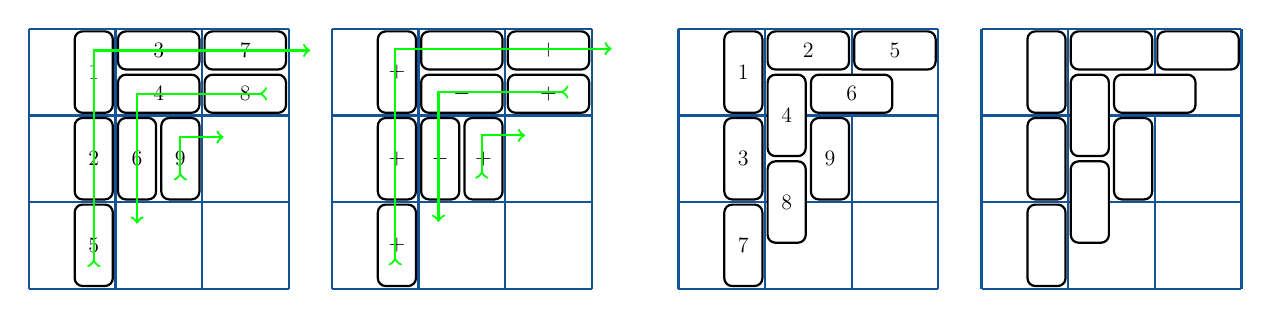
\begin{tikzpicture}[tableau, scale=.55]
      \gridLines{3}{3}\verticalDomino{1}{2}{1}\verticalDomino{3}{2}{2}\horizontalDomino{1}{3}{3}\horizontalDomino{2}{3}{4}\verticalDomino{5}{2}{5}\verticalDomino{3}{3}{6}\horizontalDomino{1}{5}{7}\horizontalDomino{2}{5}{8}\verticalDomino{3}{4}{9}
      % \fixedSquaresForGrid{3}{3}

      \draw[cycleLine] (1.5, 5.5) -- ++ (0, -5) -- + (5, 0);
      \draw[cycleLine] (5.5, 1.5) -- ++ (-3, 0) -- + (0, 3);
      \draw[cycleLine] (3.5, 3.5) -- ++ (0, -1) -- + (1, 0);

      \gridLinesShift{3}{3}{7}\verticalDominoShift{1}{2}{+}{7}\verticalDominoShift{3}{2}{+}{7}\horizontalDominoShift{1}{3}{-}{7}\horizontalDominoShift{2}{3}{-}{7}\verticalDominoShift{5}{2}{+}{7}\verticalDominoShift{3}{3}{-}{7}\horizontalDominoShift{1}{5}{+}{7}\horizontalDominoShift{2}{5}{+}{7}\verticalDominoShift{3}{4}{+}{7}
      % \fixedSquaresForGridShift{3}{3}{7}

      \draw[cycleLine] (1.5 + 7 -.04, 5.5 -.04) -- ++ (0, -5) -- + (5, 0);
      \draw[cycleLine] (5.5 + 7 -.04, 1.5 -.04) -- ++ (-3, 0) -- + (0, 3);
      \draw[cycleLine] (3.5 + 7 -.04, 3.5 -.04) -- ++ (0, -1) -- + (1, 0);

      \gridLinesShift{3}{3}{15}\verticalDominoShift{1}{2}{1}{15}\horizontalDominoShift{1}{3}{2}{15}\verticalDominoShift{3}{2}{3}{15}\verticalDominoShift{2}{3}{4}{15}\horizontalDominoShift{1}{5}{5}{15}\horizontalDominoShift{2}{4}{6}{15}\verticalDominoShift{5}{2}{7}{15}\verticalDominoShift{4}{3}{8}{15}
      \verticalDominoShift{3}{4}{9}{15}
      % \fixedSquaresForGridShift{3}{3}{15}

      \gridLinesShift{3}{3}{22}\verticalDominoShift{1}{2}{}{22}\horizontalDominoShift{1}{3}{}{22}\verticalDominoShift{3}{2}{}{22}\verticalDominoShift{2}{3}{}{22}\horizontalDominoShift{1}{5}{}{22}\horizontalDominoShift{2}{4}{}{22}\verticalDominoShift{5}{2}{}{22}\verticalDominoShift{4}{3}{}{22}\verticalDominoShift{3}{4}{}{22}
      % \fixedSquaresForGridShift{3}{3}{22}
    \end{tikzpicture}
  \end{figure}

  \tikzstyle{dominoStyle} = [color=black, fill=white, rounded corners = .1cm, thick]

\end{document}
